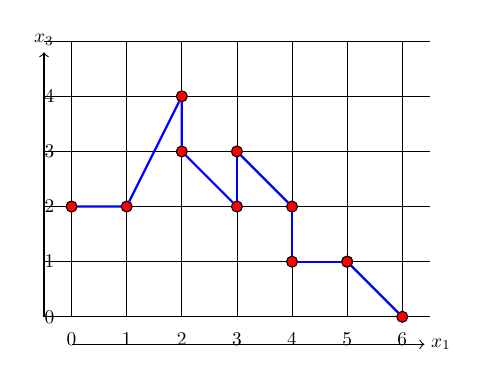
\begin{tikzpicture}[scale=0.7, transform shape]
\tikzset{
    point/.style = {
        draw,
        circle,
        inner sep = 2pt,
        fill = red
    }
}

\draw[->] (0,-0.5)--(6.4,-0.5) node[right] {$x_1$};
\draw[->] (-0.5,0)--(-0.5,4.8) node[above] {$x_3$};
\draw[line width=0.3pt, color=black] (-0.5,0) grid (6.5,5);
\foreach \x in {0,...,6}
{
    \node at (\x,-0.4){$\x$};
}
\foreach \y in {0,...,4}
{
    \node at (-0.4,\y){$\y$};
}

\node [point] (a1) at (0,2){};
\node [point] (b1) at (1,2){};
\node [point] (c1) at (2,4){};
\node [point] (d1) at (2,3){};
\node [point] (e1) at (3,2){};
\node [point] (f1) at (3,3){};
\node [point] (g1) at (4,2){};
\node [point] (h1) at (4,1){};
\node [point] (i1) at (5,1){};
\node [point] (j1) at (5,1){};
\node [point] (k1) at (6,0){};

\draw[blue, thick] (a1) -- (b1);
\draw[blue, thick] (b1) -- (c1);
\draw[blue, thick] (c1) -- (d1);
\draw[blue, thick] (d1) -- (e1);
\draw[blue, thick] (e1) -- (f1);
\draw[blue, thick] (f1) -- (g1);
\draw[blue, thick] (g1) -- (h1);
\draw[blue, thick] (h1) -- (i1);
\draw[blue, thick] (i1) -- (j1);
\draw[blue, thick] (j1) -- (k1);

\end{tikzpicture}